\section{{{\fontsize{17}{21}\selectfont \textbf{Introduction}}}}
\setlength{\columnsep}{1.5cm}
\begin{multicols}{2}
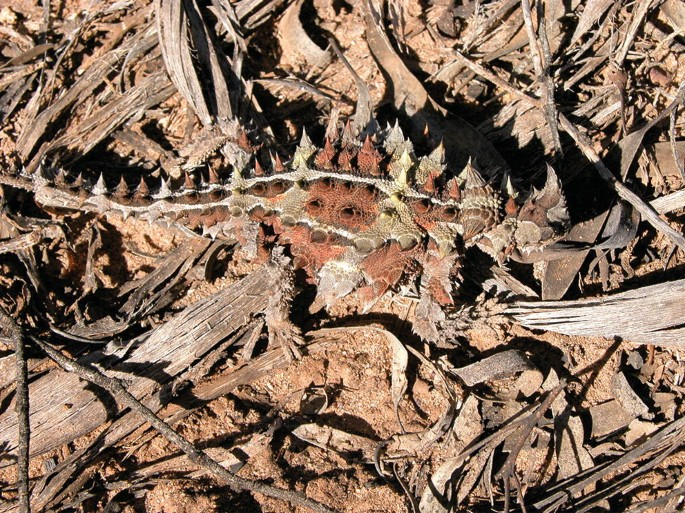
\includegraphics[width=\columnwidth,height=8cm]{sections/LBP/418993_0_En_698-1_Fig1_HTML.jpg}
\captionof{figure}{Example of background matching camouflage (BMC)}
\vspace{0.5cm}
 The given example as referred by Biologists is Background Matching Camouflage (BMC), where one or more objects attempt to adapt their coloring to match "seamlessly" with the surroundings in order to avoid detection. Naturally, addressing concealed object detection (COD) requires a significant amount of visual perception knowledge. Understanding COD has not only scientific value in itself, but it is also important for applications in many fundamental fields, such as computer vision, medicine, agriculture, and art.\\
 In our project we have use SINet architecture for detecting camouflaged objects. The SINet model is a state-of-the-art architecture for image classification that can detect both RGB\cite{OBJ_DET} and multispectral images. The model uses a deep convolutional neural network that learns and extracts features from the input image. The extracted features are then processed and classified using a fully connected layer.\\
 However, the SINet model is based on 3-input channels, which limits its capability to process multispectral images with more than 3 spectral bands. To overcome this limitation, we use Principal Component Analysis (PCA) to convert multispectral images with 5 spectral bands to 3 featured images. This conversion allows us to use the SINet model to detect camouflaged objects in multispectral images with more than 3 spectral bands.\\
 We trained our model using drone data, which provides a realistic representation of the environment where camouflage detection is of utmost importance. The drone data consists of high-resolution images captured from different angles and heights, which helps our model to learn and generalize better.\\
\end{multicols}

\vspace{0.5cm}
{\color{gray}\hrule}
\vspace{0.5cm}